\PassOptionsToPackage{table,dvipsnames,svgnames}{xcolor}
\documentclass[portrait,final,a0paper]{nadiposter}

\usepackage{fontawesome}

\selectcolormodel{RGB}

\usepackage{graphicx}
\usepackage{multicol}
\usepackage{sectsty}

\usepackage{pgfbaselayers}
\pgfdeclarelayer{background}
\pgfdeclarelayer{foreground}
\pgfsetlayers{background,main,foreground}

\usepackage{amssymb}% http://ctan.org/pkg/amssymb
\usepackage{pifont}% http://ctan.org/pkg/pifont
\newcommand{\cmark}{\textcolor{blue}{\ding{51}}}%
\newcommand{\xmark}{\textcolor{red}{\ding{55}}}%
\newcommand{\pointer}{\scalebox{2}{\ding{43}}}%
% \usepackage{tikz}
% \def\checkmark{\tikz\fill[scale=0.4](0,.35) -- (.25,0) -- (1,.7) -- (.25,.15) -- cycle;}

%%%%%%%%%%%%%%%%%%%%%%%%%%%%%%%%%%%%%%%%%%%%%%%%%%%%%%%%%%%%%%%%%%%%%%%%%%%%%%%%
% Multicol Settings

\setlength{\columnsep}{1.5em}
\setlength{\columnseprule}{0mm}

%%%%%%%%%%%%%%%%%%%%%%%%%%%%%%%%%%%%%%%%%%%%%%%%%%%%%%%%%%%%%%%%%%%%%%%%%%%%%%%%


% ----------------------------------------------------------------------- %

% Useful hints
% https://tex.stackexchange.com/questions/252757/including-boxes-inside-boxes-in-baposter

% ----------------------------------------------------------------------- %



\newcommand{\compresslist}{%
\setlength{\itemsep}{1pt}%
\setlength{\parskip}{0pt}%
\setlength{\parsep}{0pt}%
\setlength{\leftmargin}{0pt}%
}


\contactInfo{%
\begin{tabular}{c}
  Viet Minh Vu, Adrien~Bibal and Beno\^it~Fr\'enay \\
  \faEnvelopeO\ : \{vuvietminh, adrien.bibal, benoit.frenay\}@unamur.be \\
%   \faGlobe\ : staff.info.unamur.be/jmj
\end{tabular}}



\begin{document}

\definecolor{unamurgreen}{RGB}{69,181,63}
\definecolor{unamurgray}{RGB}{64,68,67}
\definecolor{lightunamurgreen}{RGB}{69,181,63}

% from poster example

\definecolor{lightorange}{rgb}{0.9,0.4,0}
\definecolor{lightestorange}{rgb}{1,0.8,0.5}
\definecolor{darkorange}{rgb}{0.2,0.1,0}

% end from poster example


\typeout{Poster Starts}


\begin{poster}%
  % Poster Options
  {
  % Show grid to help with alignment
  % grid=true,
  grid=false,
  % Column spacing
  colspacing=1em,
  % Color style
  bgColorOne=lightunamurgreen,
  bgColorTwo=white,
  borderColor=unamurgray,
  headerColorOne=unamurgray,
  headerColorTwo=lightorange,
  headerFontColor=white,
  boxColorOne=white,
  boxColorTwo=white,
  % Format of textbox
  textborder=roundedright,
  % Format of text header
  eyecatcher=true,
  headerborder=closed,
  headerheight=0.1\textheight,
%  textfont=\sc, An example of changing the text font
  headershape=roundedleft,
  headershade=plain,
  headerfont=\Large\bf\textsc, %Sans Serif
  textfont={\setlength{\parindent}{1.5em}},
  boxshade=plain,
  background=plain,
  linewidth=2pt,
  columns=4
  }
  % Eye Catcher
  {\hbox{} } %
\includegraphics[height=7em]{images/nadi-red.png}} 
  % Title
  {\bf\textsc{Tuning of Visualization Algorithms\\*[0.3em] with User Constraints for $t$-SNE}\vspace{0.5em}}
  % Authors%   Viet~Minh~Vu,  Adrien~Bibal, Beno\^it~Fr\'enay
  {\textsc{Viet Minh Vu, Adrien~Bibal,  Beno\^it~Fr\'enay} } % \\ {Universit\'e de Namur - Faculty of Computer Science}
  % University logo
  {% The makebox allows the title to flow into the logo, this is a hack because of the L shaped logo.
   \hbox{} % 
\includegraphics[height=7em]{images/nadi-red.png}
  }


% --------------------------------------------------------------------------- %

\sectionfont{\centering}

% --------------------------------------------------------------------------- %
\headerbox{Difficulty in choosing a good parameter for a visualization algorithm (t-SNE)}{name=intro,column=0,row=0,span=4}{

\begin{minipage}{0.63\linewidth}   
    \begin{center} \Large{\textbf{Problematic and Motivation}} \end{center}
    
    \begin{tabular}{p{3.cm} p{11.cm}}
        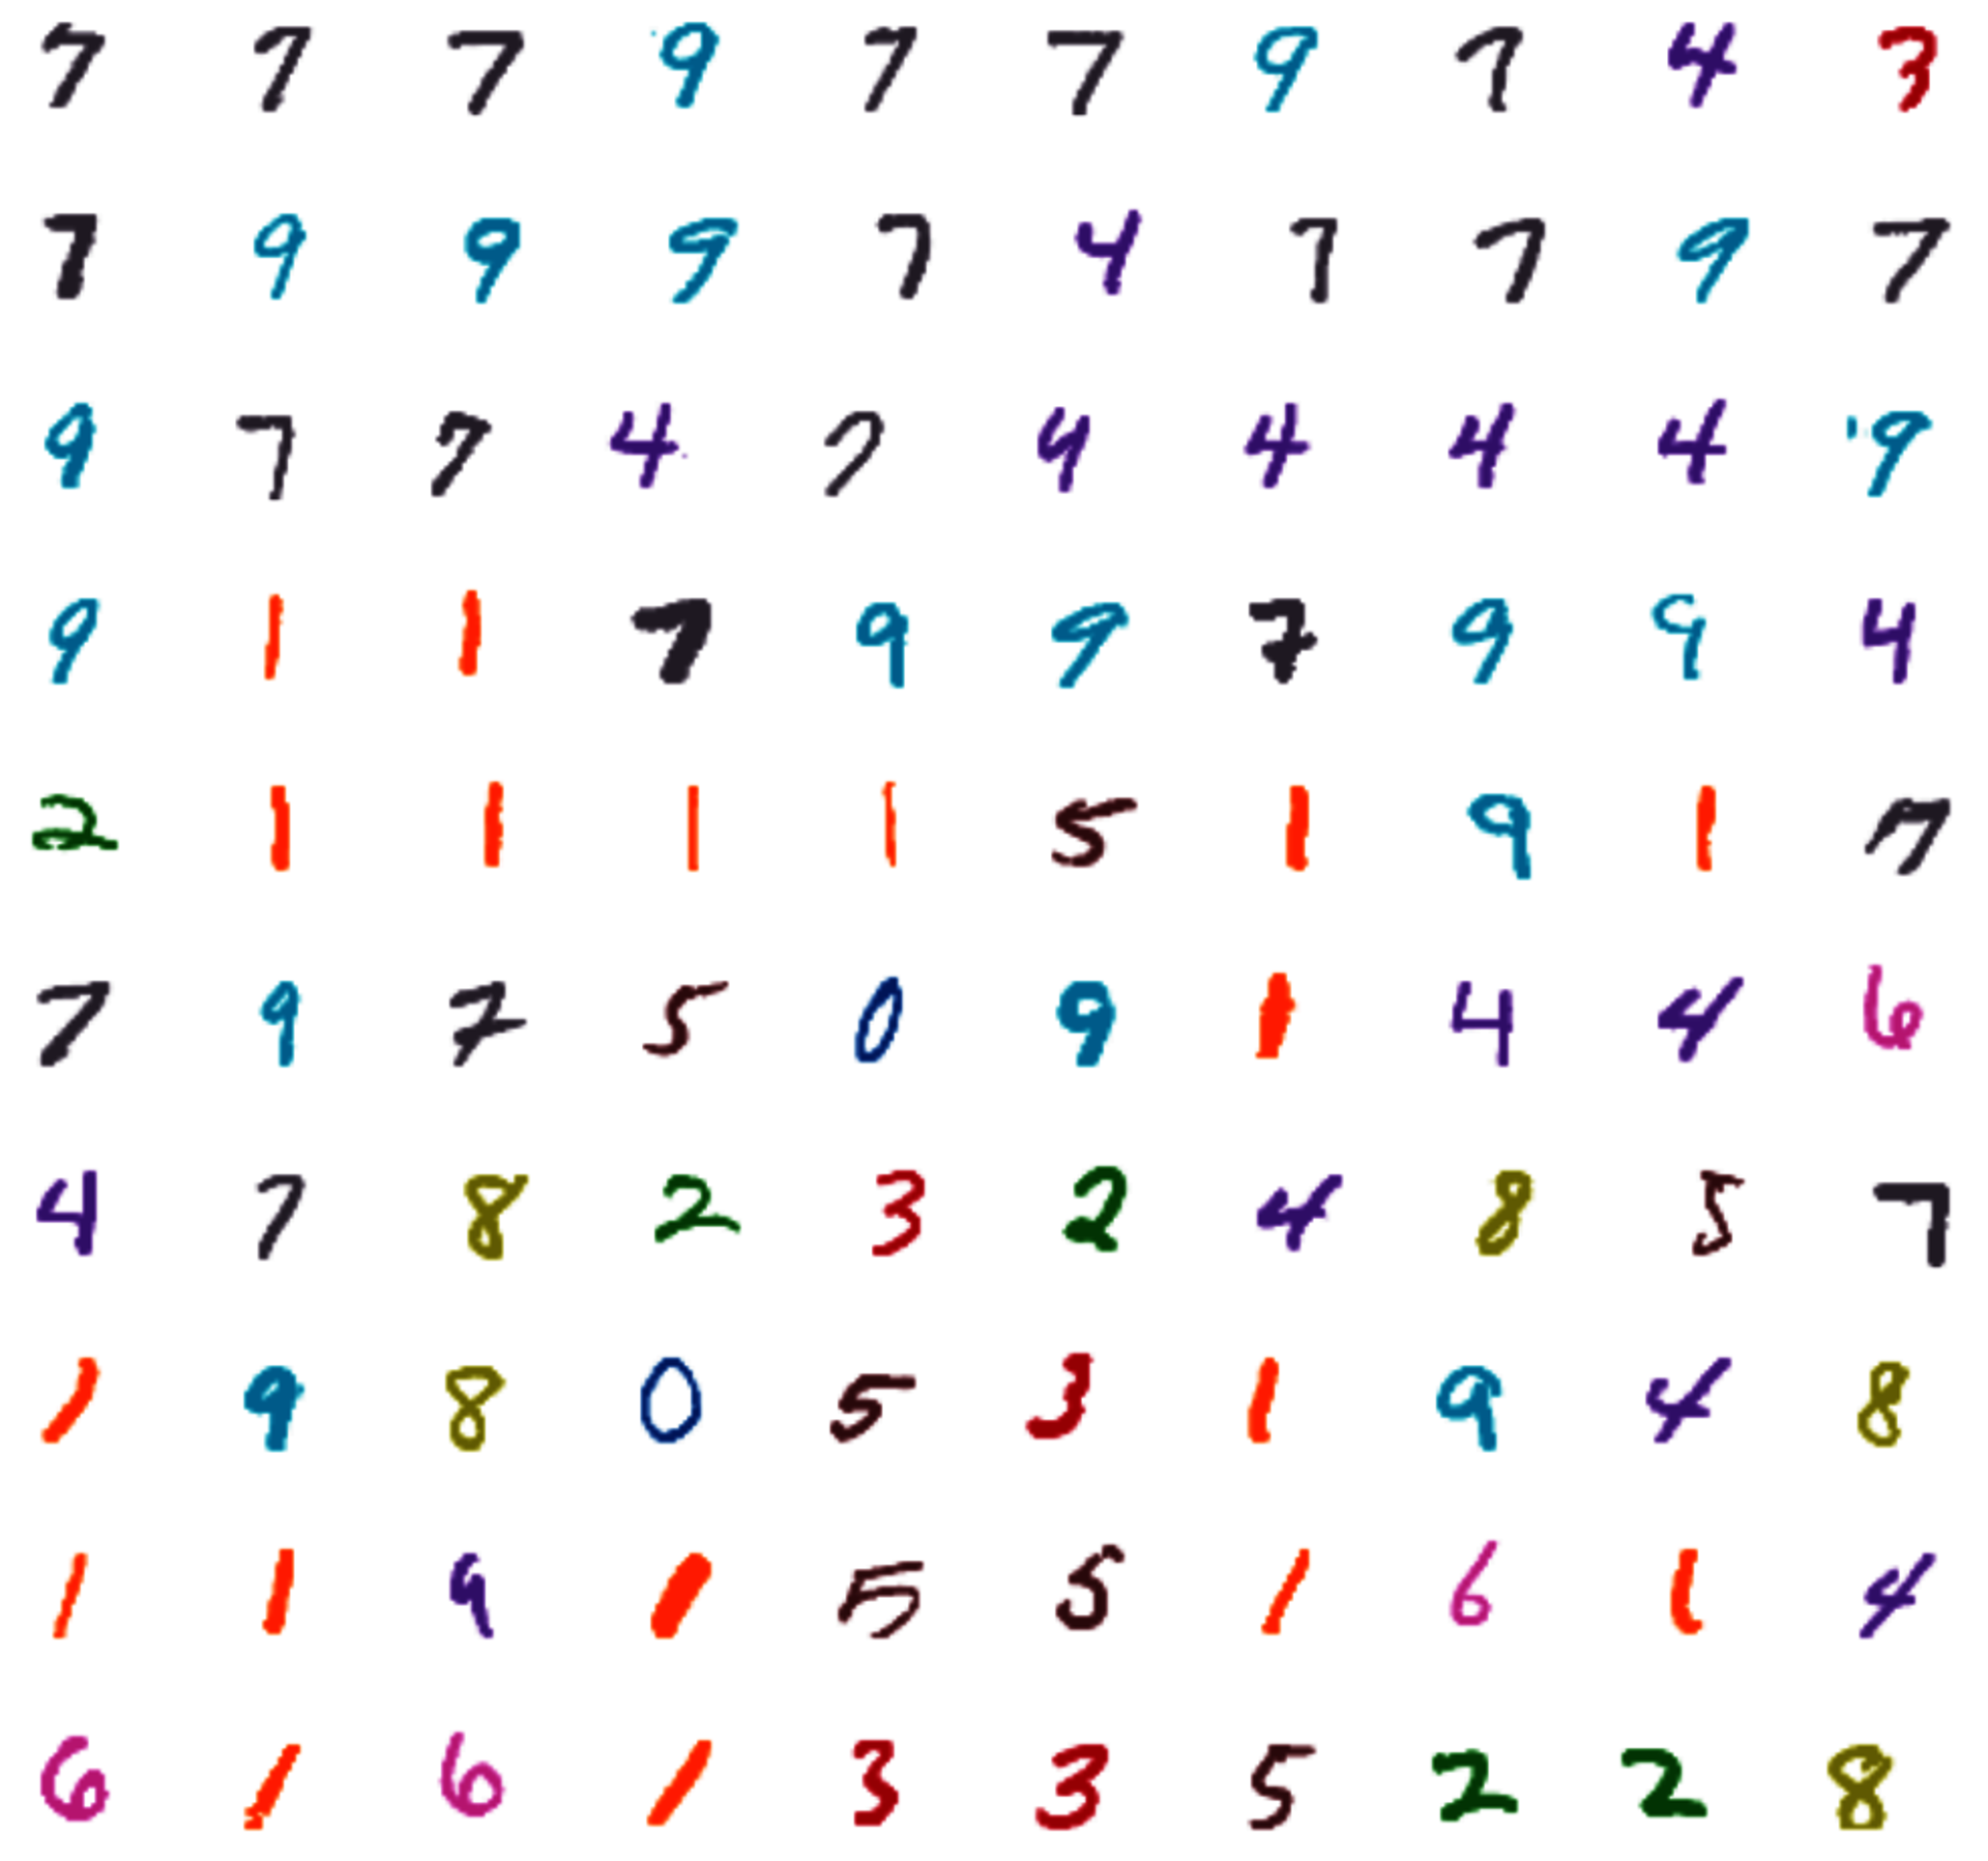
\includegraphics[height=8em]{images/mnist_raw200.pdf}&
        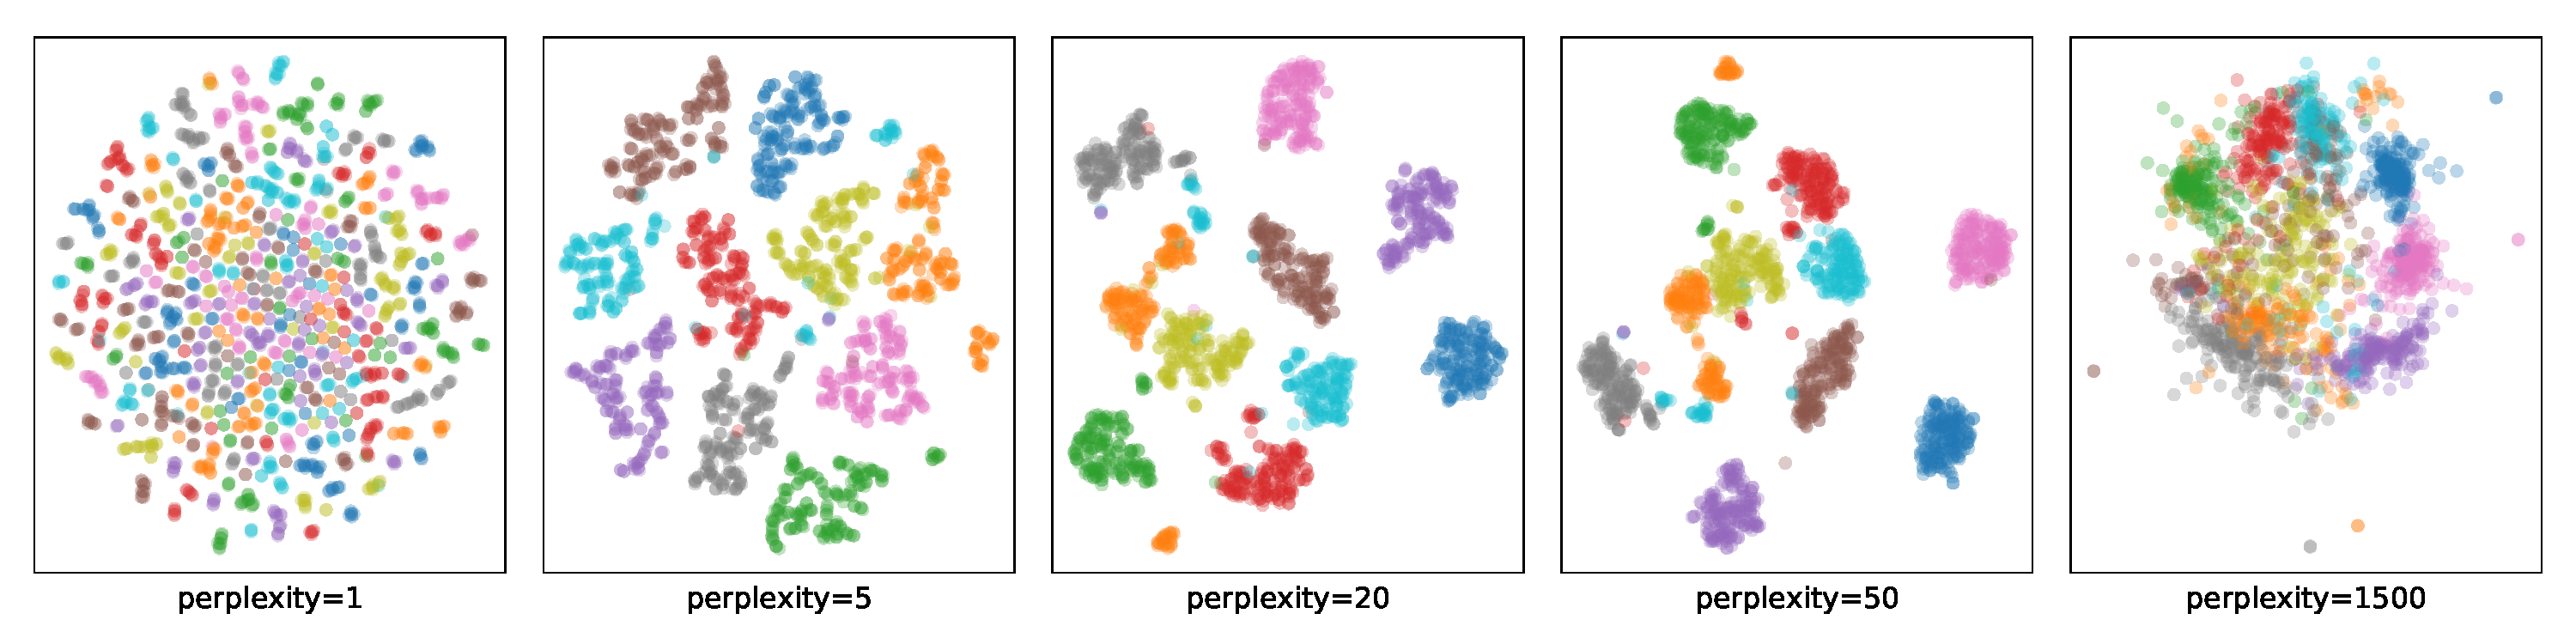
\includegraphics[height=8em]{images/MNIST-SMALL_examples.pdf}\\
        Goal: Visualize the \scriptsize{\textbf{high~dimensional}~data}&
        t-SNE is sensitive to the \emph{perplexity} parameter, which is \textbf{important} but very \textbf{hard to understand and to tune}.\\
    \end{tabular}
\end{minipage}
\begin{minipage}{0.33\linewidth}
    \begin{center} \Large{\textbf{Proposed Solution}}\end{center}
    $\;$Use the users' \textbf{feedback} to \textcolor{blue}{steer the visualization}.
    
    \begin{itemize}
        \compresslist{
            \item Let users define their requirements in form of \textbf{pairwise constraints}\textcolor{blue}{[A]} between examples.
            \item The \emph{perplexity} is automatically chosen based on the user's \textbf{constraint scores}\textcolor{blue}{[B]}.
            \item Evaluate the proposed visualization by quantitatively comparing with the state-of-the-art \textbf{quality metrics}\textcolor{blue}{[C]}.
        }
    \end{itemize}
\end{minipage}
}

% --------------------------------------------------------------------------- %
\headerbox{User pairwise constraints \textcolor{white}{[A]}}{name=constraint_gui,column=0,span=4,below=intro}{
\begin{multicols}{2}
    \section*{\large{What are expressed by user (in high dim.)}}
    \begin{center}
    \begin{tabular}{c}
        Two \textcolor{blue}{similar} examples $\rightarrow$ \textcolor{blue}{\textbf{Must link}}.\\
        Two \textcolor{red}{dissimilar} examples $\rightarrow$ \textcolor{red}{\textbf{Cannot link}}. \\
        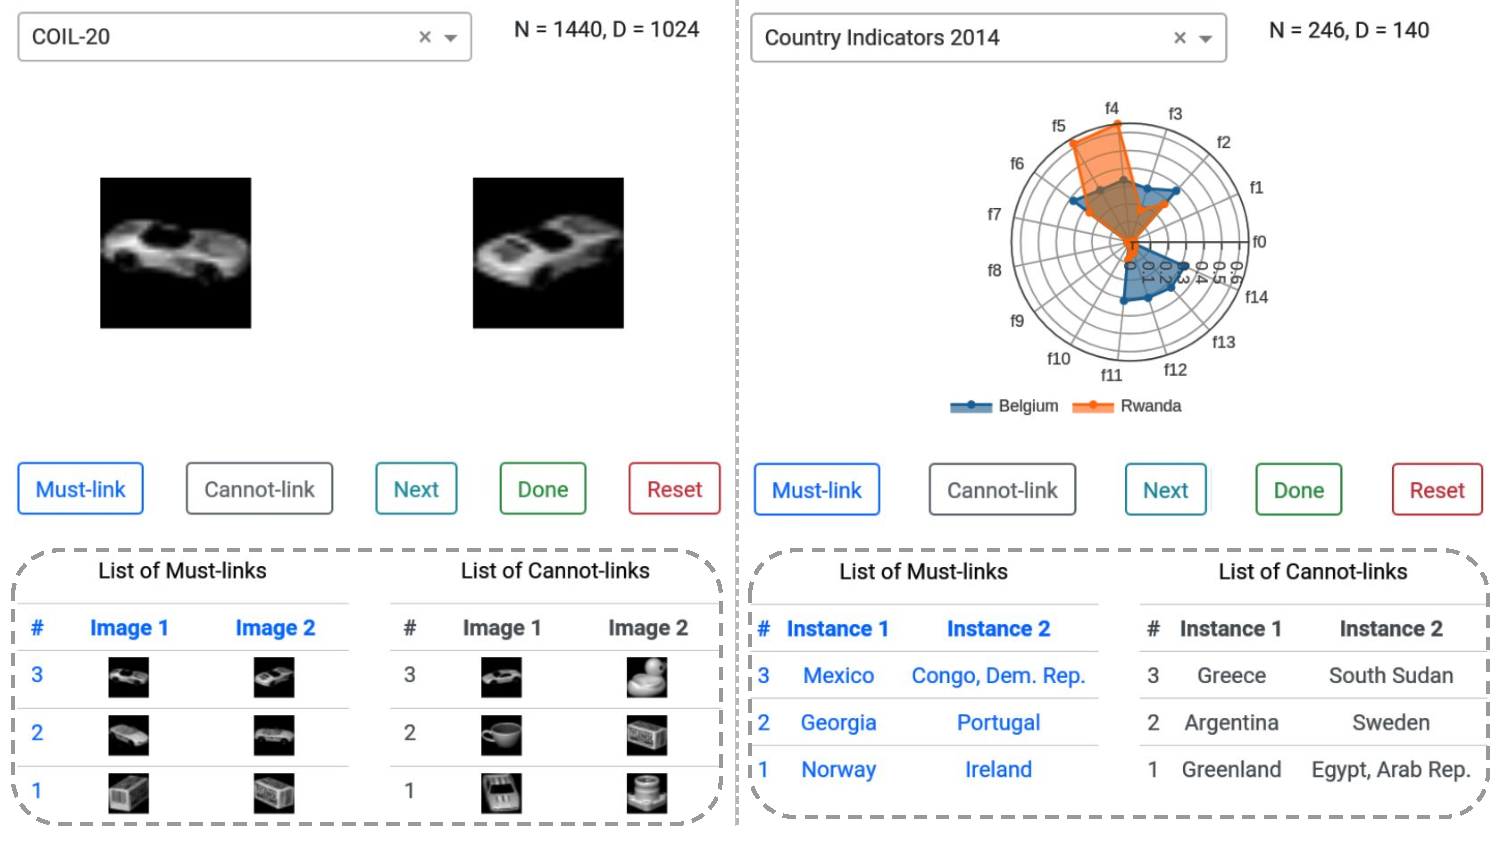
\includegraphics[height=12.5em]{poster_NADI_2018/images/app_guis_no_annotations.pdf}\\
        \tiny{Figure: The interface for collecting the users' feedback.}
    \end{tabular}
    \end{center}
    \section*{\large{What are translated to the algorithm (in low dim.)}}
    \noindent
    \begin{center}
    \begin{tabular}{c}
        Points connected by a \textcolor{blue}{\textbf{Must link}} $\rightarrow$ must stay \textbf{close together}.\\
        Points connected by a \textcolor{red}{\textbf{Cannot link}} $\rightarrow$ must stay \textbf{far apart}.\\
        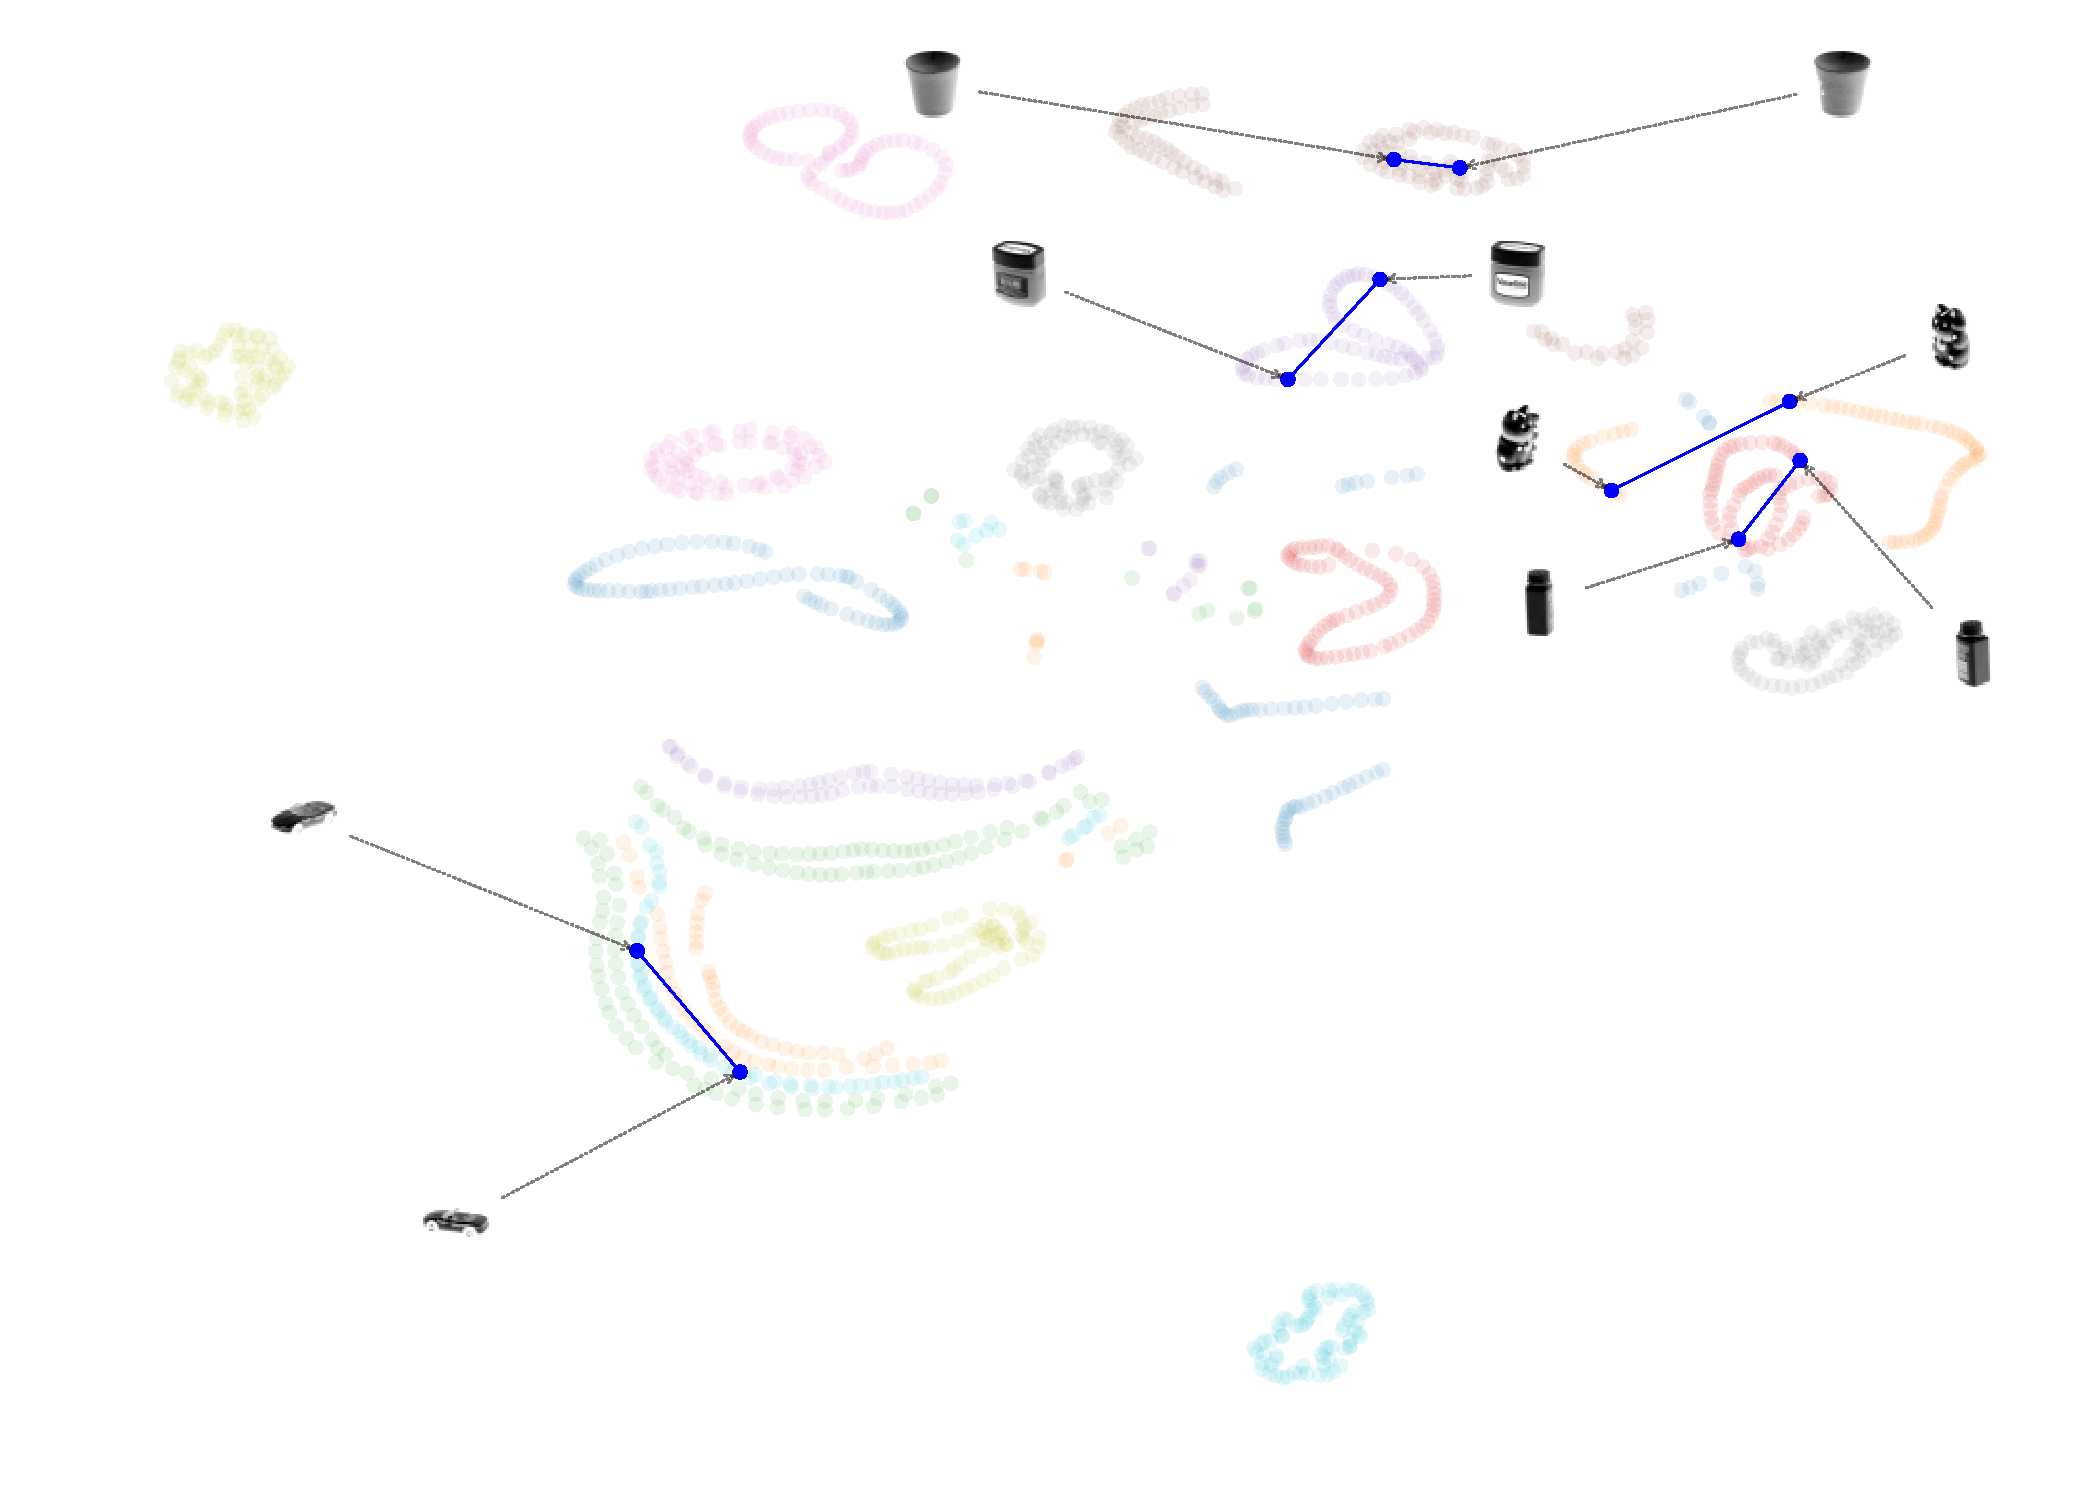
\includegraphics[height=12em]{poster_NADI_2018/images/example_constrains_COIL20_ML.pdf}
        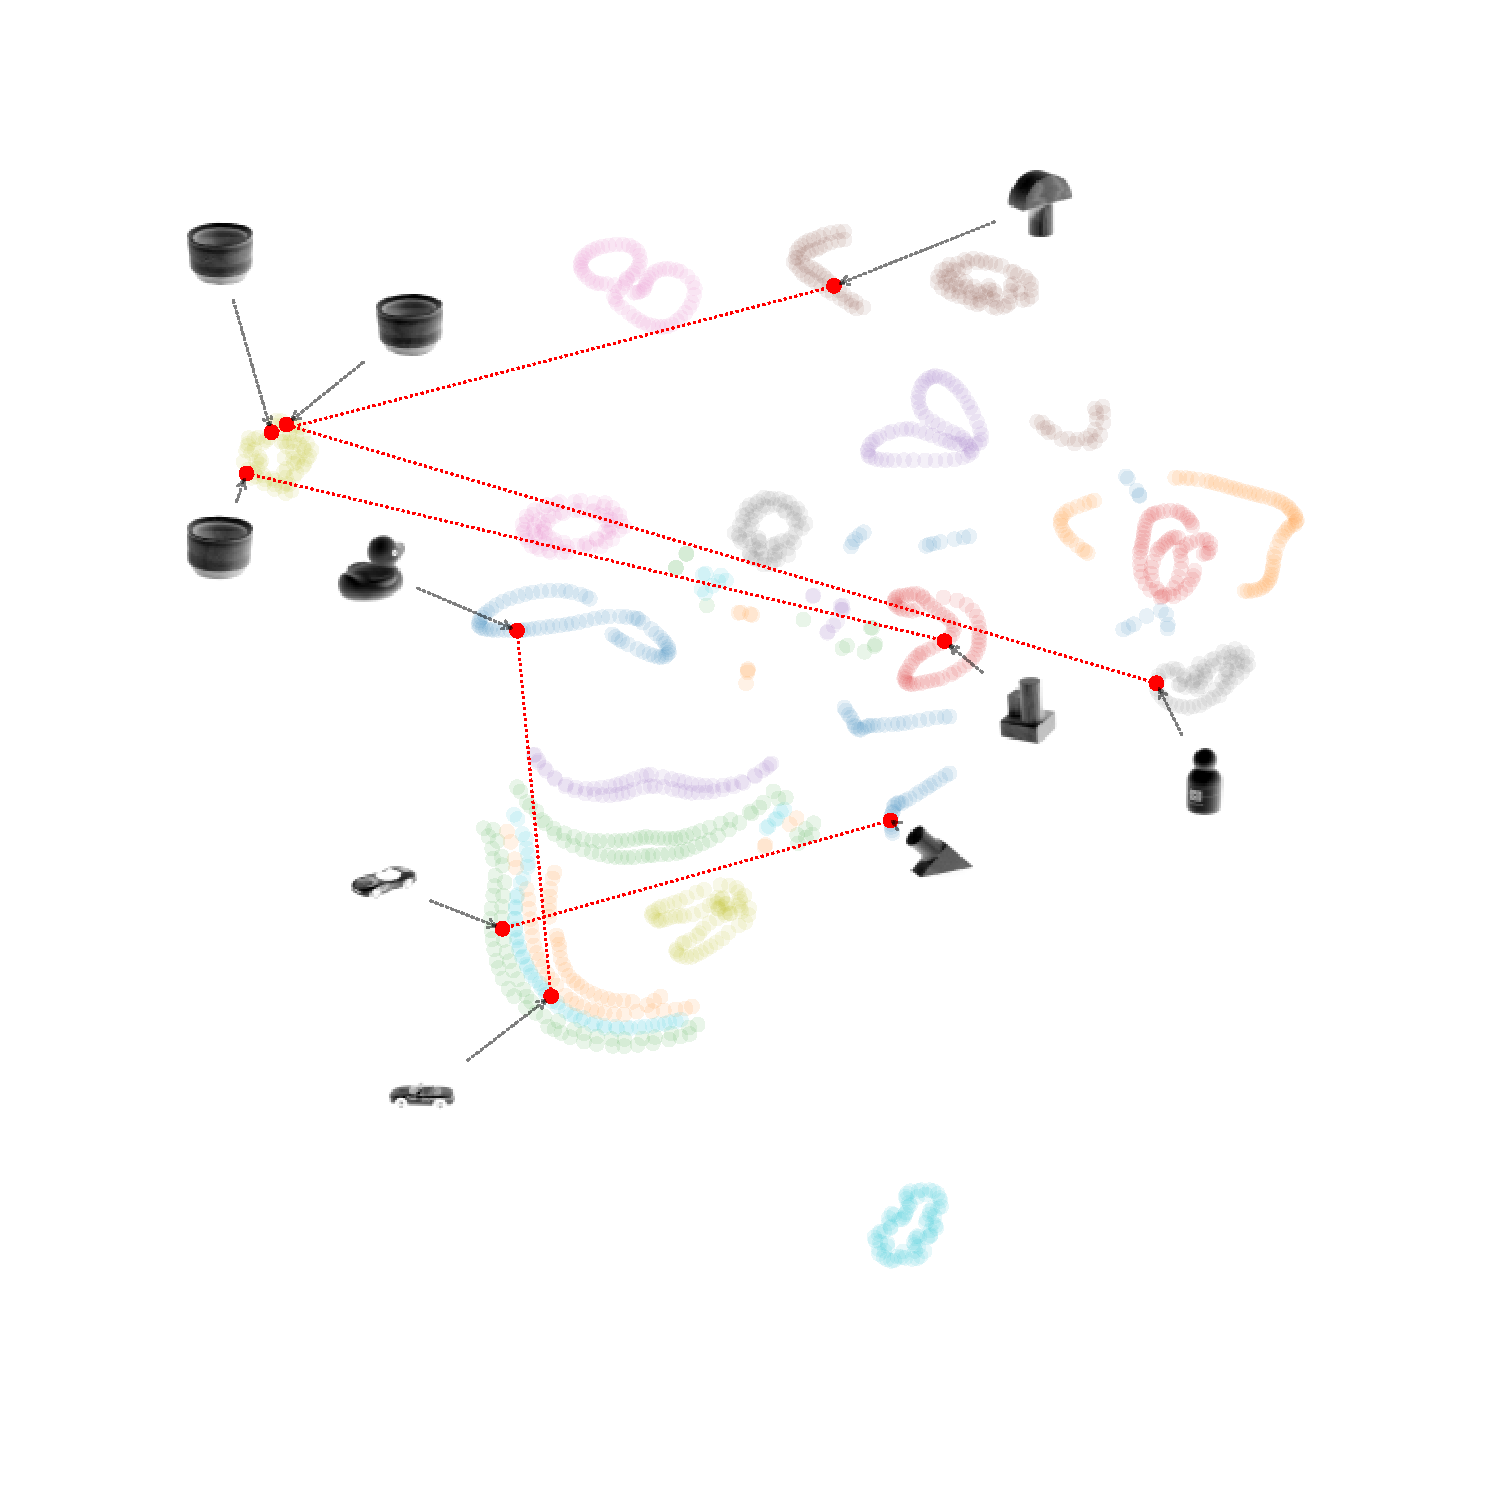
\includegraphics[height=12em]{poster_NADI_2018/images/example_constrains_COIL20_CL.pdf}\\
        \tiny{Figure: The user constraints in the visualization (COIL20 dataset).}
    \end{tabular}
    \end{center}
\end{multicols}
}

% --------------------------------------------------------------------------- %
\headerbox{Constraint-Preserving Scores \textcolor{white}{[B]}}{name=constraint_score,column=0,span=2,below=constraint_gui}{
\noindent
\begin{minipage}{0.48\linewidth}
    \begin{itemize}
        \compresslist
        \item Consider the points in the visualization (low dim.)
        \item $q_{ij} = $ probability of $i$ and $j$ being neighbors.
    \end{itemize}
    \begin{itemize}
        \item \textcolor{blue}{$S_{\mathcal{M}} = \frac{1}{|\mathcal{M}|} \sum_{(i,j) \in \mathcal{M}} \log q_{ij}.$}
        \item \textcolor{red}{$S_{\mathcal{C}} = -\frac{1}{|\mathcal{C}|} \sum_{(i,j) \in \mathcal{C}} \log q_{ij}.$}
        \item \textcolor{BurntOrange}{$S_{\mathcal{M}+\mathcal{C}} = S_{\mathcal{M}} + S_{\mathcal{C}}.$}
    \end{itemize}
\end{minipage}
\begin{minipage}{0.48\linewidth}
    \begin{center}
    \begin{tabular}{c}
        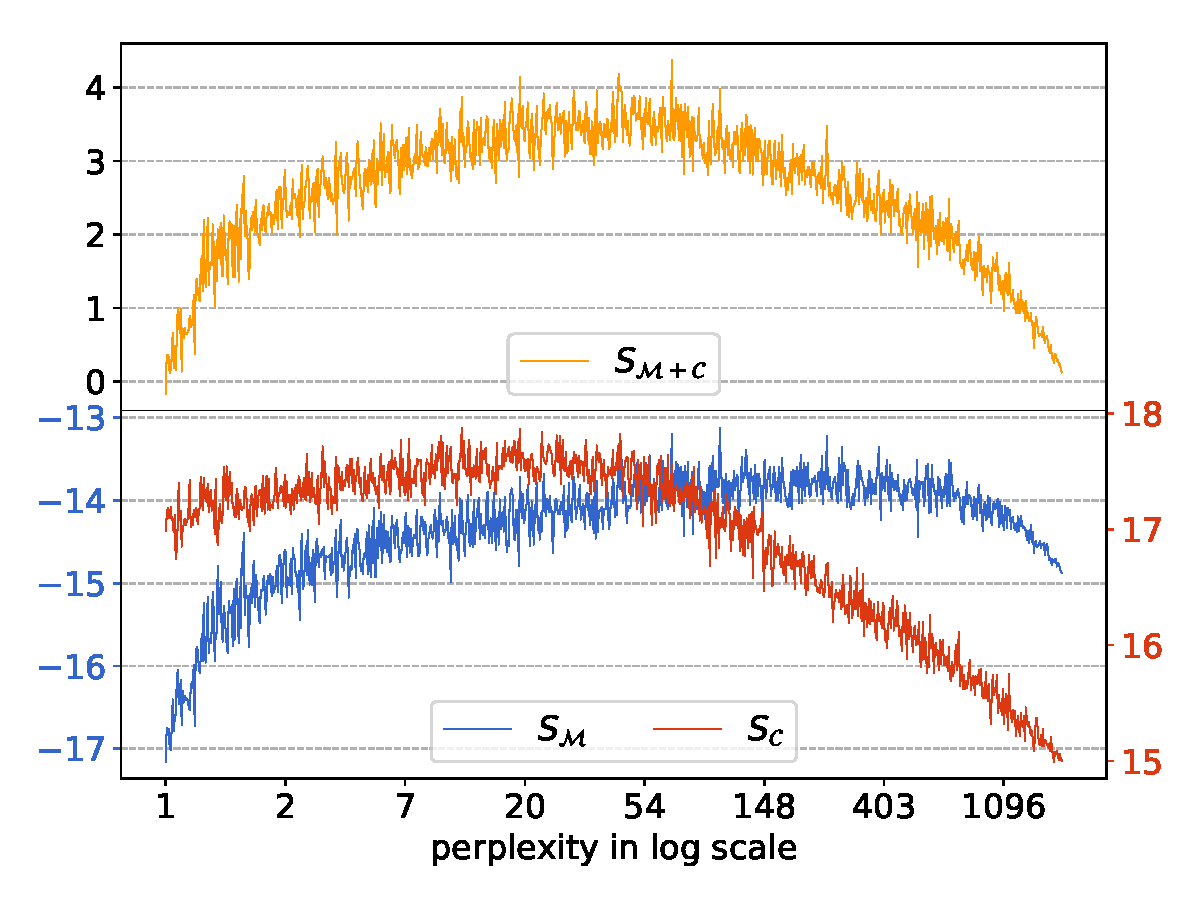
\includegraphics[height=11em]{poster_NADI_2018/images/s_scores_50.pdf}\\
        \tiny{Figure :Constraint-preserving scores}\\
        \tiny{with 50 constraints for MNIST dataset.}
    \end{tabular}
    \end{center}
\end{minipage}

\noindent
\pointer \quad \fbox{Can easily find the perplexity that maximizes \textcolor{blue}{$S_{\mathcal{M}}$}, \textcolor{red}{$S_{\mathcal{C}}$} or \textcolor{BurntOrange}{$S_{\mathcal{M}+\mathcal{C}}$}.}
}

% --------------------------------------------------------------------------- %
\headerbox{Quality Metrics\textcolor{white}{[C]}}{name=metrics,column=2,span=2,below=constraint_gui}{
\noindent
\begin{minipage}{0.48\linewidth}
    \begin{itemize}
        \compresslist
        \item \textbf{CC}: Pearson corr. coeff.
        \item \textbf{NMS}: Stress of pairwise distance orders comparison
        \item \textbf{CCA}: Stress with accent put on low dim.
        \item \textbf{NLM}: Stress with accent put on high dim.
        \item \textcolor{NavyBlue}{\textbf{AUC$_{log}$RNX}}: Neighbors-preserving in low dim.
    \end{itemize}
\end{minipage}
\begin{minipage}{0.48\linewidth}
    \begin{center}
    \begin{tabular}{c}
        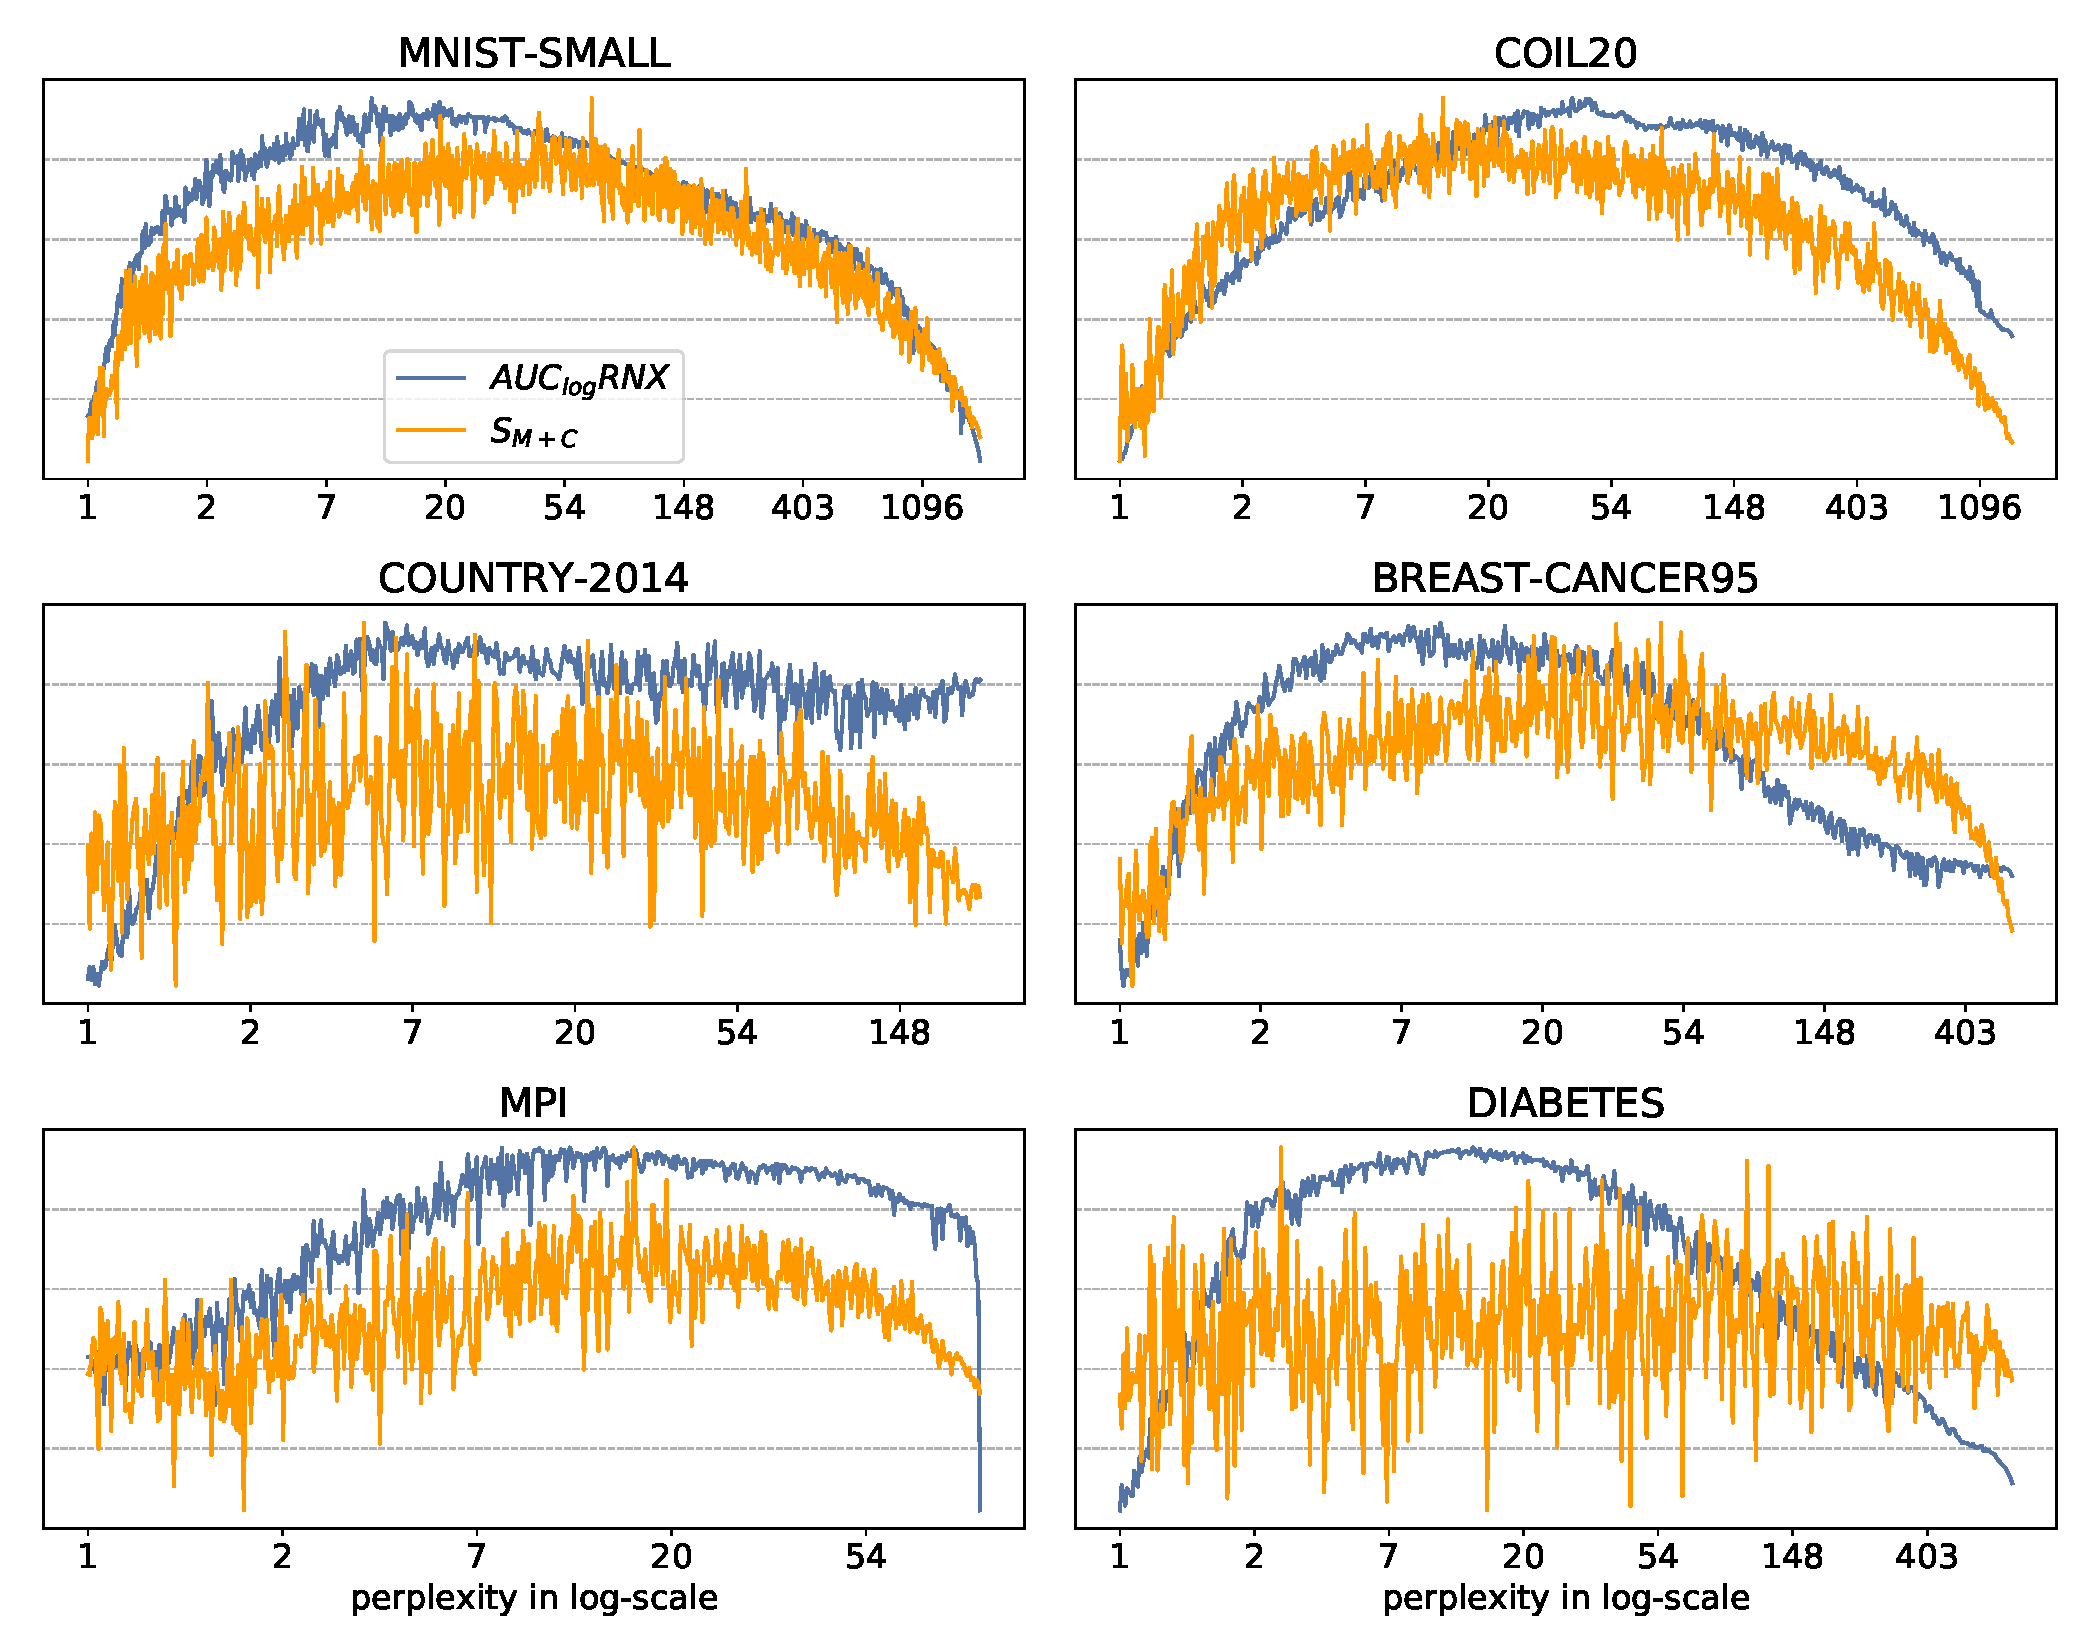
\includegraphics[height=10em]{poster_NADI_2018/images/sall_auc_50.pdf}\\
        \tiny{Figure: Compare \textcolor{BurntOrange}{$S_{\mathcal{M}+\mathcal{C}}$} and \textcolor{NavyBlue}{\textbf{AUC$_{log}$RNX}}}\\
        \tiny{for six datasets.}
    \end{tabular}
    \end{center}
\end{minipage}

\vspace{1.em}
\noindent
\pointer \quad \fbox{Our constraint scores agree with the quality metrics.}
}

% --------------------------------------------------------------------------- %
\headerbox{All the visualizations in one place: Meta-plot}{name=metaplot,column=0,span=3,below=constraint_score}{
\begin{center}
\begin{tabular}{c}
    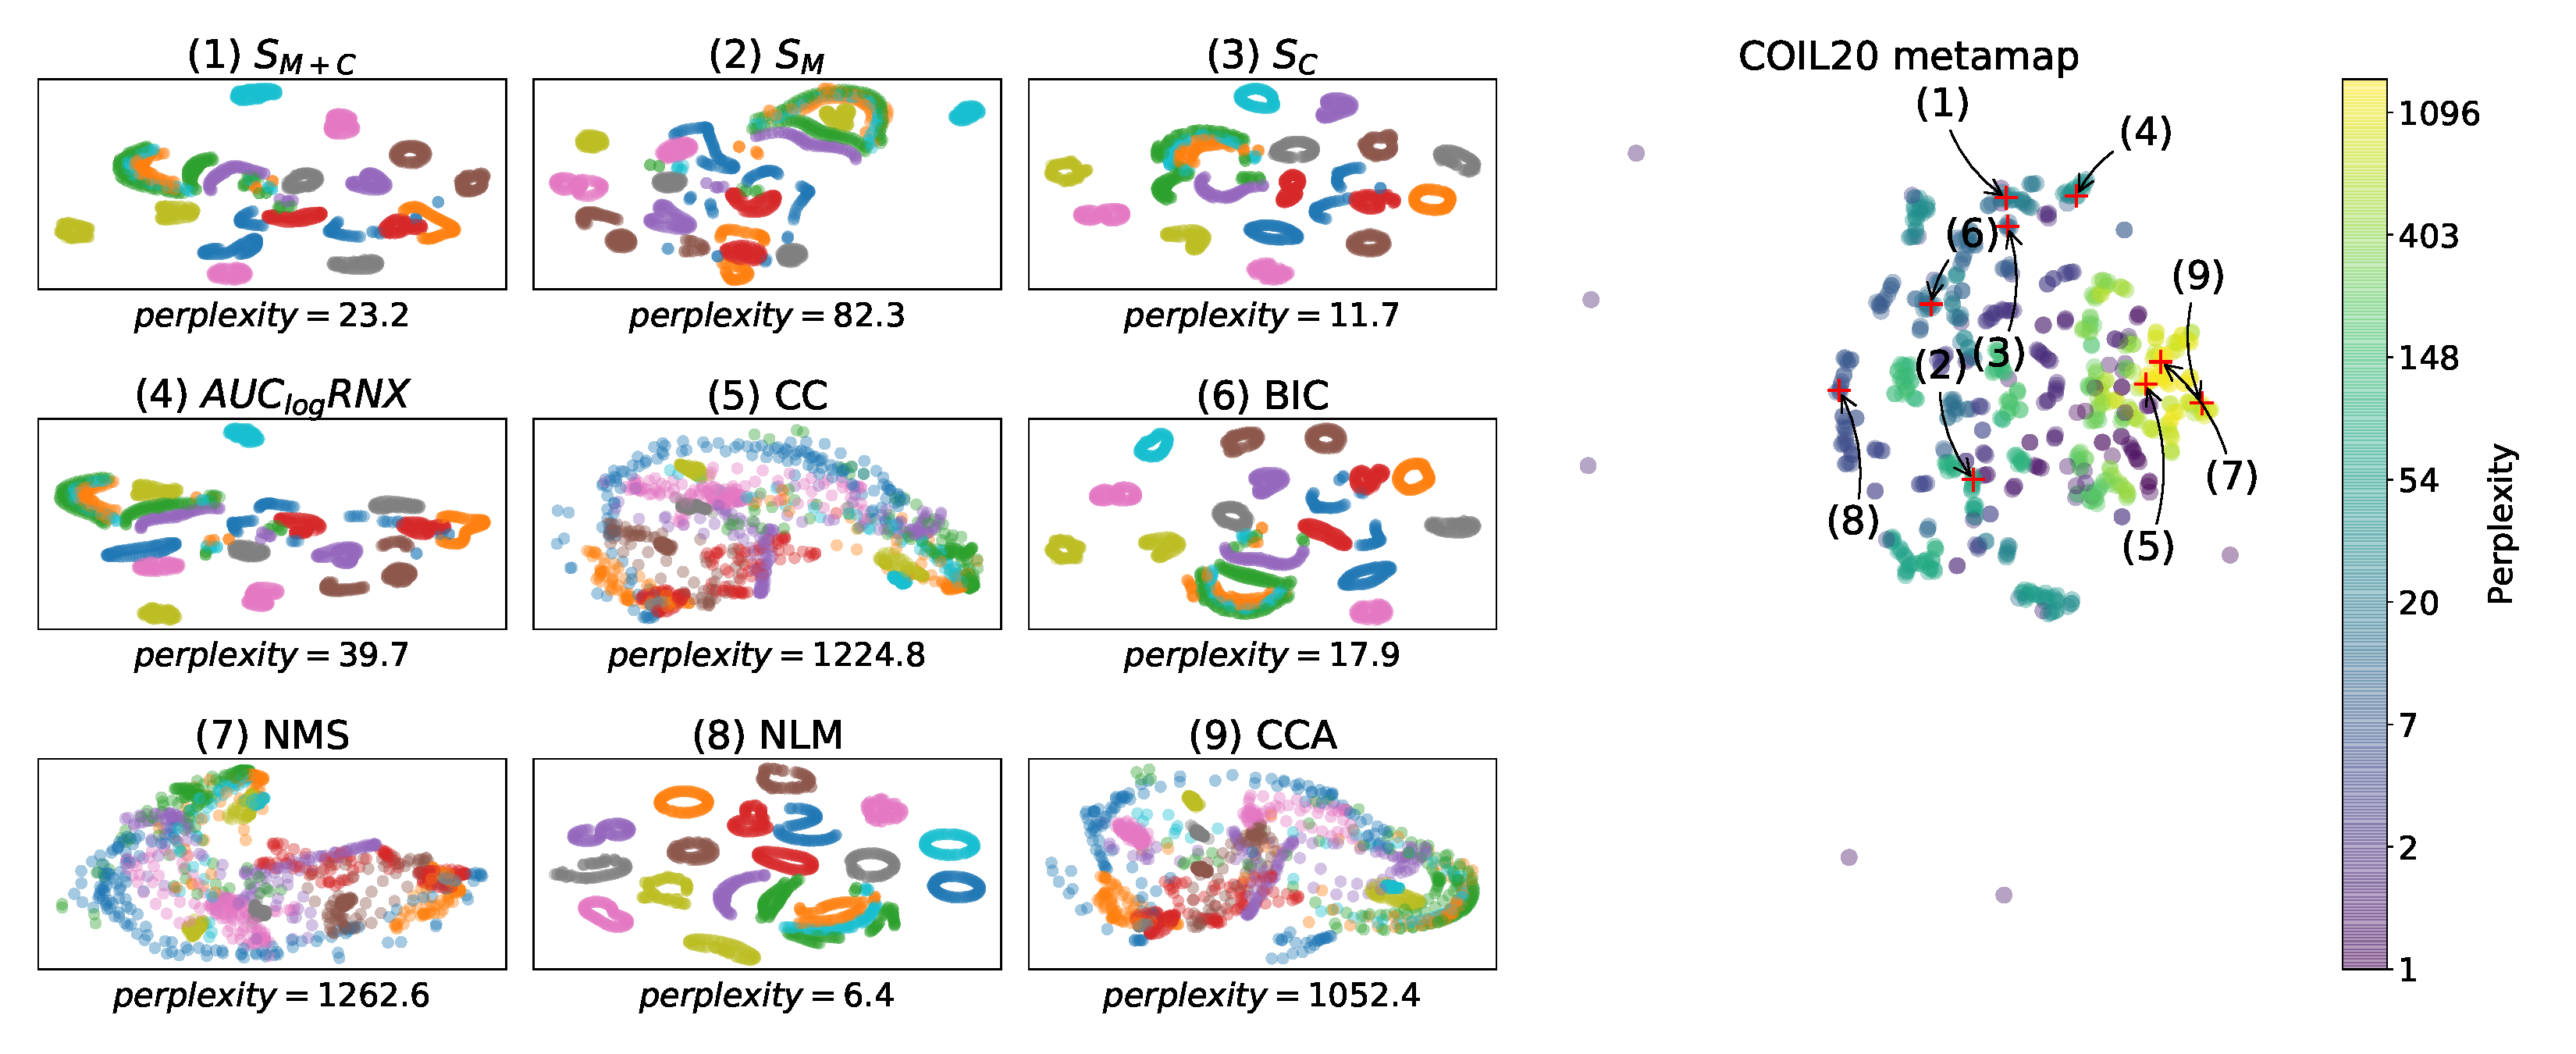
\includegraphics[height=16em]{poster_NADI_2018/images/COIL20_meta.pdf}
\end{tabular}
\end{center}
}


% --------------------------------------------------------------------------- %
\headerbox{Conclusion}{name=conclusion,column=3,span=1,below=constraint_score}{
\noindent
\cmark \quad Consider \emph{user knowledge} under the form of constraints to find the most suitable visualization.

\vspace{0.75em}
\noindent
\cmark \quad Make complex visualization technique ($t$-SNE) \emph{accessible} to users by freeing them from the tedious task of selecting the hyper-parameter.

\vspace{1.25em}
\noindent
\xmark \quad \emph{Heavy computation} due to the pre-calculation of all the embedding and the greedy approach for searching the optimal perplexity.
}

\end{poster}

\end{document}

